\documentclass[../TDO3.tex]{subfiles}%

\begin{document}
\section[s]"2"{Coin de miroir}
\QR{%
	Un rayon lumineux pénètre dans un système optique composé de deux miroirs plans
	faisant un angle $\alpha$ entre eux. Il rentre parallèlement à un
	miroir et ressort du système en revenant sur lui-même par le même chemin
	optique après trois réflexions. Quelle est la valeur de $\alpha$~?
}{%
	~
	\smallbreak
	\vspace{-15pt}
	\noindent
	\begin{minipage}{0.48\linewidth}
		On compte 3 réflexions, et il doit revenir sur lui-même~: le rayon incident
		et le rayon émergent doivent faire le même angle avec la normale à BC.
		L'angle $i_2$ est également identique de $I$ à $J$ et de $J$ à $I$. Cela
		n'est vérifié que si la lumière est en incidence normale sur AB.

		Or, $i_1 = \frac{\pi}{2} - \alpha$, donc $i_2 = -i_1 =
			\alpha-\frac{\pi}{2}$. Pour avoir $i_2$ dirigé verticalement, il faut
		$-i_1+i_2 = -\frac{\pi}{2}$, autrement dit $2i_1 = \frac{\pi}{2}
			\Leftrightarrow i_1 = \frac{\pi}{4}$. Finalement, on trouve

		\begin{empheq}[box=\fbox]{equation*}
			\alpha = \SI[parse-numbers=false]{\frac{\pi}{4}}{rad}
		\end{empheq}
	\end{minipage}
	\hfill
	\begin{minipage}{0.48\linewidth}
		\begin{center}
			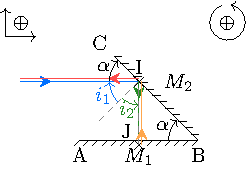
\includegraphics[width=\linewidth]{coin_mir}
			\captionof{figure}{Schéma du système}
			\label{fig:coin_mir}
		\end{center}
	\end{minipage}
}

\end{document}
